\AUTChapter{Literature Review} \label{chap:litrev}

\section{Introduction}\label{sec:Introduction}

The literature review design of this PHD research constitutes of 3 parts, 2 systematic literature reviews (SLR) on the topics ‘Big data reference architectures’ and ‘E-commerce systems” and one generic literature review on the topic ‘Big data’.

Systematic literature reviews take shape by embarking on an extensive search for topic-related articles within the years 2010-2020. Most literature chosen for the purposes of this research are within the years 2016-2020 as they provided with recent, and more relevant information. Albeit, some old studies dating back to 2010, helped clarifying some basic matters that existed and how they correlated to big data. world most renowned online libraries for quality research have been selected such as IEEE, MIS Quarterly, Science Direct, Elsevier, Springer, ACM, AISeL and Emerald insight.

Every library provided with a vast sea of research and inordinate amount of information to absorb. Arguably, different publications provided with different sort of mental framework and so did the authors. For instance, it’s been found that many high-quality information system researches are published in MIS quarterly, whereas Elsevir and SpringerLink provided with quality big-data literature.

A combination of long-tail and short-tail keywords are chosen to target literature that are related to the current state of art. Keywords chosen for ‘Big data reference architectures’ SLR are ‘big data reference architectures’, and ‘reference architectures. Keywords chosen for ‘E-commerce systems’ are ‘e-commerce system architectures’, ‘smart e-commerce systems’, and ‘e-commerce and big data’. Each systematic literature review is conducted in a span of three weeks.

In what follows, first the generic big data literature review will be conducted, second ‘big data reference architecture’ SLR and finally ‘E-commerce systems’ SLR will take place.

\section{State of the art}\label{sec:State of the art}

We’ve come a long way with technology, and specifically software development. In fact, the rapid advancements left many spaced out. From the emergence of the first computer Eniac in 1946 to 8-core 5.0GHz processing core speed in 2019; From document-oriented waterfalls to agile two-weeks sprints; from punch cards to fancy transpilers  and dynamic programming languages.  Computers were first perceived as calculation engines and has been used to focus entirely on algorithms and mathematics. It was during the mid-1950, that it became commercially available and businessmen start to pick it up to produce value for business. Along the lines, once people started using computers for real-life purposes, many leftover data has been produced, as these data increased, people started realizing the value of it and began to store it \cite{Grad2009}.

That’s where the industry came up with a concept of a Database Management System (DBMS), and humanity began to store data for various purposes. In 1968, as a result of a NATO-sponsored conference, the term software engineering emerged, referring to a highly systematic approach to software development and maintenance \cite{Wirth2008}.

Since the beginning of 1968, the advancement began on the areas of tools generation, testing, automation and systematizing. During the same years, in 1960s the history of computer hardware started by conversion of vacuum tubes to solid-states. Todays, the word ‘bug’ is quite a common phrase among engineers and programmers to refer to a fault, failure or a flaw. We ow this word to a literal moth that were caught inside a tube before the transition to solid states. It is hardly conceivable that we’ve progressed from absolutely no understanding for data to devices that can produce zettabytes of them in a span of 60 years. Along this track, software engineering has passed several major phases. Recent polyglot approaches with nascent lambda functions, functional paradigms and micro-services have come to take the industry by storm. This is the only time in human history, where the computing resources and the necessary data is available to harness the hidden patterns behind every momentum or dynamism. Being so focused on development of more maintainable and scalable software, and microchips and hardware’s and devices that can perform faster and last longer, we have lost the track of the output of all these entities and peripherals, and that’s the void that current industry is facing. Abundance of computer power, the emergence of open source community, and the ubiquity of internet has brought us with a new material to harness. A material, that is complex and random in nature.

It was not until 2005 that the term big data has been coined \cite{Long2015}, and Web 2.0 emerged which referred to a large set of data that is impossible to process with the traditional data management systems. Within the same year, Yahoo created Hadoop, Google came up with MapReduce. In 2009, the Indian government took a revolutionary step and decided to take an iris scan of its 1.2 billion inhabitants. In 2011 McKinesy published the title “Big Data: the next frontier of innovation” and startups and companies started investing heavily in this field. The big data revolution is ahead of us, and yet there is a big chasm both in practice and academia \cite{mckinsey2011big}.

\footnote{A transpiler is a sort of a compiler that translates source codes from one language to another, or another version of the same language. For example Babel (a Javascript Library ) transpiles the latest syntax of Javascript ( ES6 ) into older version of it ( ES5 ), thus all the browsers can support the system.}

\section{Big data}\label{Big Data}
\subsection{What is big data?}\label{What is big data?}

To define big data for the course of this PHD thesis, we will first look at available definitions in academia.

\citeauthor{Kaisler2013} define big data as “the amount of data which is beyond technology’s capability to store, manage and process efficiently.\citeauthor{Srivastava2018} referred to big data as “the use of large data sets to handle the collection or reporting of data that serves business or other recipients in decision making”.

\citeauthor{Sagiroglu2013} define big data as “a term for massive data sets having large, more varied and complex structure with the difficulties of storing, analyzing and visualizing for further processes or results”.  Inspired by these definitions, we define big data as “an endeavor to harness the patterns behind vast amount of data for the purposes of improvement, control, and prediction of business matters”.

\section{The Hype of Emerging Technologies}

The term big data, was initially coined to refer to the gradual growth and availability of data \cite{lycett2013datafication}.

The ubiquity of digital devices and capability of users to produce different forms of data, have consolidated the interconnected links among suppliers, customers, affiliates, partners, and stakeholders \cite{Bughin2016}. With recent emergence of 5G technology and its launch in the UK, we are experiencing a fundamental network shift that is unprecedented in human history \cite{ahmad20205g}

Opposed to general belief of 5G being only faster than its elder brother 4G, 5G has come to offer bi-directional large bandwidth shaping, large broadcasting of data in gigabits which supports wearable devices with AI capabilities, pervasive networks providing ubiquitous computing (the user can be seamlessly connected to several wireless access technologies), traffic statistics, IPV6 utilization and finally 25Mbps of connectivity speed \cite{Gohil2013}.

In a world where we have the average processing power of 1.5 GHz on smart phones and up to 8 GHz on desktops running on network infrastructures that will support up to 25Mbps of transmission per second, data becomes the new oil, the atom, the dot that lays the foundation of the nexus \cite{Rad2017}. It is astonishing to witness data being produced by netizens in every second .According to live internet statistics website , there are 4 billion internet users currently active, that produce 8,522 Tweets, 920 Instagram photos, 1,540 Tumbler posts, 3,868 Skype calls, 74,993 Google searches, 79,099 Youtube videos, 2,806,143 emails, and 73,693 GB of internet traffic per second \cite{Stats2017}. That implies, if it has taken 3 seconds to read the preceding paragraph, in the interim, 221,79 GB of traffic has been produced. Howbeit, how useful are these data? And how far have we gone with harnessing its power?


\section{The Value of Big Data}

The value of big data is no longer under the hood. In fact, the concept has been repeatedly discussed in various reports, statistics, researches and conferences \cite{Chen2012}. The outburst is driven by the colossal investment of companies such as Google, Facebook, Netflix and Amazon \cite{Rada2017}.

A study of Netflix Prize recommender system provided details on employment of big data in order to induce better, more accurate results \cite{Amatriain2013}. The research has explicitly stated the notion of using various pools of data to further optimize recommendations. Data produced by queries, ratings, queues, search terms, and metadata alongside impression, social, external, demographic, location, language, and finally temporal data has been taken in use for predictive models \cite{Amatriain2013}. Using big data enforced recommendation systems, the company has managed to increase TV series consumption by the factor of four \cite{Amatriain2013}.

The Taiwanese government leveraged its national health insurance database and merged it with custom and immigration datasets to forge a big data initiative \cite{wang2020response}. This initiative resulted in improved case identification by generating real-time alerts during clinical visits. These alerts have been created by the analysis of clinical symptoms, travel history, and other data that could be found. Proactively seeking out patients that may be infected by COVID-19 was one of the reasons that Taiwanese government managed to handle the epidemic effectively.

Shell uses big data to reduce costs energy resources exploration \cite{Marr2016}. The company uploads data to analytics system and compare it with data from drilling sites around the world. The closer the results match where abundant resources have been found, the better decision will be made. Before big data, company had huge problems to identify energy resources. Waves of energies traveled through the earth’s crust registered differently on sensors, depending on whether they are travelling through gaseous material, liquids, or solid rocks. Formerly, company employed the traditional hit and miss approach to confirm the findings of the initial survey which was expensive and time-consuming.

Along the lines, Rolls Royce harness the power of big data by capturing internal data from sensors fitter on the company’s aircraft products. The data is received through a wireless transmission medium and contains multitudes of performance reports. These reports shed lights on various key phases such as take-off, engine power climax, steady state (climb and cruise), dynamisms, and maintenance \cite{Marr2016}. The company uses the data to detect degradation, to induce diagnosis and prognosis, and to minimize the false-positive as well.

\section{Datocracy}

The availability of data at an unprecedented frequency and the hidden patterns behind this nexus of interconnections has resulted in a new world, a datocratic world. Before getting further, is it essential to grasp the meaning of the new term ‘Datocracy’ proposed to correctly address the lingual needs for this research. To clarify the meaning of the word, it is helpful to understand the etymology behind the common term “Democracy”. Deomcracy comes from the combination of two ancient Greek words namely “demos” meaning ‘people’, and the post fix “-Kratia” meaning ‘to rule’. By the same line the combination of the Greek word “Datum” and the post fix “-Kratia” generates the word Datocracy, meaning “data to rule”.


\begin{figure}[h!]
    \centering
    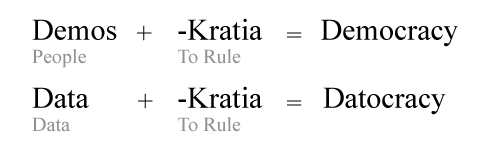
\includegraphics[width=8cm]{Datocracy.png}
    \caption{Datocracy}
    \label{fig:datocracy}
\end{figure}


\section{Ubiquity}

Recent technology shifts and the computing power that each person carries along, has brought along a new business material, a datocracy. In a conference held in Abu Dhabi in 2013, Joseph S. Nye, a former US assistance secretary of defense and a university professor at Harvard, proposed the idea of future governance in the age of information \cite{Nye2013}.

He proposed the scenario in which the central government will use big data to fortify control. On the other hand, there is an estimation of 7121 publications on the fields big data regarding different dimensions, such as mathematical techniques, decision-making techniques, data characteristics, technical challenges and adoption failures \cite{Wang2016}.

Paying clear attention to recent social, commercial and industrial trends will yield the evidence of big data ubiquity. In the domain of social network, there has been study for understanding temporal patterns of happiness by using a data set of 46 billion words contained in nearly 4.6 billion expression by 63 million unique users posted over a 33 months span \cite{Dodds2011}.

Furthermore, in another research, big data analytics and semantic network analysis were utilized to examine the largest data set collected on Twitter during 2012 U.S presidential election \cite{Guo2015}. The study concluded that the news media could determine the public’s identification of a certain candidate.

Other academicians have used big data to develop a novel distributed community structure mining framework. The framework makes use of local information data alongside MapReduce, and well-known algorithms such as FastGN, and Radetal to address scalability, velocity, and accuracy \cite{Jin2015}. On a bigger, more social-oriented studies, there has been researches regarding the overall well-being Turkish citizens by adopting a sentiment analysis model \cite{Durahim2015}.

Along the lines, the very sentiment analysis model has been taken by other researchers to discover general knowledge from social media \cite{Bohlouli2015}, and to evaluate and infer enhanced marketing advantage and to shed lights on areas in which the business is leading and lagging to further improve customer-business relation \cite{He2015}.

Similar researches have been conducted by analyzing suspended spam accounts on Twitter in terms of the profile’s properties and interactions. These researchers were aimed to point out spammers and malicious users by using big data \cite{Almaatouq2016}. \citeauthor{Chainey2008} have conducted a research on hotspot mapping and its usage to identify spatial patterns of crime. The study concluded that by utilizing a data from the past, hotspot mappings can identify where crimes most densely occur. From there on, there has been the proposition of target enforcement and prevention resources in the crime areas for mitigating crimes.

By the same token, \cite{Li2012} used a large dataset from the bank of Taiwan and developed a big data system to identify signs and patterns of fraudulent accounts. They’ve developed a detection system by applying the Bayesian Classification and Association Rule. Along the lines, there has been other researches to predict negative behaviors spreading dynamics \cite{Liao2015}, emotional response detection by browsing Facebook \cite{Lin2015}, as well as identifying the impacts of national security by using the US intelligent community datasets \cite{Crampton2015}.

A wander into different areas provides with interesting ideas about how far the progress has been with the adoption of big data and proves a truly datocratic world. One good example is a comparative study conducted to document how big data can help with multifaceted aspects of international accreditations for two universities, namely Plekhanov Russian University of Economic and HAN University of Applied Science (Arnhem Business School) \cite{Popescu2019}.

In addition, \cite{Zhang2019a} conducted a research on the application of big data for tours and creative agencies. The objective of the study was to extract behavioral data and to form strategic objects that can be later applied for business benefit.

As witnessed hereinabove, there are abundant number of researches on the application of big data in various industries. Table 1 portrays an overview of the aforementioned studies and even further.

\begin{center}
    \renewcommand{\arraystretch}{1.5}
    \begin{longtable}{|p{4cm}|p{8cm}|p{1cm}|}
        \caption{my caption}                                                                                                                                                                                                     \\
        \hline
        Contibution                & \multicolumn{2}{c|}{Multi-column}                                                                                                                                                           \\
        % ROW
        \hline
        \cite{Luo2016}             & Application of big data in health care                                                                                                        & \multirow{10}{*}{\begin{turn}{-90} \textit{Healthcare} \end{turn}} \\

        % ROW
        \cite{Murdoch2013}         & Adoption of big data in health care                                                                                                           &                                             \\

        % ROW
        \cite{Zhang2015}           & Application of big data in cloud in healthcare cyber-physical system                                                                          &                                             \\

        % ROW
        \cite{Zhang2015}           & Application of big data in cloud in healthcare cyber-physical system                                                                          &                                             \\

        % ROW
        \cite{Bates2014}           & Exerting big data analytics to identify and manage high-risk and high-cost patients                                                           &                                             \\

        % ROW
        \cite{Lin2016}             & Designing systems for emotion-aware healthcare using big data                                                                                 &                                             \\

        % ROW
        \cite{Lin2016}             & Designing systems for emotion-aware healthcare using big data                                                                                 &                                             \\

        % ROW
        \cite{Srinivasan2013}      & Analyzing health insurance claims to detect frauds, errors, waste, abuse                                                                      &                                             \\

        % ROW
        \cite{Mehta2018}           & Analysis of application of big data in healthcare                                                                                             &                                             \\

        % ROW
        \cite{firouzi2018internet} & Amalgamation of Internet of Things (IoT) and Big Data for a smarter healthcare                                                                &                                             \\

        % ROW
        \cite{firouzi2018internet} & Analysis of application of big data in healthcare                                                                                             &                                             \\

        % ROW
        \cite{Chen2018}            & Analysis of application of big data in healthcare                                                                                             &                                             \\

        % ROW
        \hline
        \cite{asur2010predicting}  & Predictive analytics using social networks                                                                                                    & \multirow{5}{*}{\begin{turn}{-90} \textit{Social} \end{turn}}  \\

        % ROW
        \cite{Dodds2011}           & Revealing temporal patterns of happiness                                                                                                      &                                             \\

        % ROW
        \cite{Guo2015}             & Utilizing big data to examine message networks such as Twitter and traditional news media                                                     &                                             \\

        % ROW
        \cite{Jin2015}             & Developing a novel distributed community structure mining framework                                                                           &                                             \\

        % ROW
        \cite{Durahim2015}         & Analysis of overall happiness in Turkey through twitter analysis and big data                                                                 &                                             \\

        % ROW
        \cite{Bohlouli2015}        & Knowledge discovery from big data                                                                                                             &                                             \\

        % ROW
        \hline
        \cite{Chainey2008}         & Predicting of spatial patterns of crime using big data                                                                                        & \multirow{1}{*}{\begin{turn}{-90} \textit{Crime and Fraud} \end{turn}}  \\

        % ROW
        \cite{Li2012}              & Using bank data to identify patterns of fraud                                                                                                 &                                             \\

        % ROW
        \cite{Liao2015}            & Predicting abusiveness in online commentaries and preventing them                                                                             &                                             \\

        % ROW
        \cite{Tran2018}            & Data driven approaches for credit card fraud detection                                                                                        &                                             \\

        % ROW
        \hline
        \cite{Sigala2019}          & A book on big data and how it can bring innovation to tourism business                                                                        & \multirow{5}{*}{\begin{turn}{-90} \textit{Tourism} \end{turn}}  \\

        % ROW
        \cite{Zhang2019a}          & Analyzing the application of big data in tourism                                                                                              &                                             \\

        % ROW
        \cite{Dezfouli2018}        & Developing a tour model using big data                                                                                                        &                                             \\

        % ROW
        \cite{Qin2019}             & Utilization of big data with Call Detail Record (CDR) data and mobile real-time location data to monitor the tourist flow and travel behavior &                                             \\

        \hline
    \end{longtable}
\end{center}


\section{Business Benefits and Challenges}

Big data and the  benefits it brought along has resulted in new approaches of decision-making, which can be called data grounded decision-making \cite{Comuzzi2016} or a datocratice decision-making.These new organizational adaptations target compelling interventions in both internal and external aspects, especially in areas that has formerly been dominated by gut and intuition rather than by data and exactitude \cite{Wamba2017}.

As the data-oriented strategies, philosophies, artifacts, technologies, tools, and methodologies emerge, they will revolutionize long-established ideologies toward the nature of decision-making, business process management, and predictive models \cite{Popovic2018}.

There is and will be a colossal attention toward the undeniable benefits of big data to lay out customer’s behavioral patterns, experimental orientation, organizational functions, business acumen, predictive decision-making, and a far more informative business and marketing plans comparing to traditional resolutions \cite{Driest2016}.

But as with any other great change, there comes the hurdles. Aside from the technical difficulties and talent shortage, turning into a data-based management, or data grounded decision-making system, would require a clear vision to align business objectives with insights, and there arise a big possibility for error \cite{Ranjan2019}.

To invest in such hype as big data and to extract insights sounds fundamentally important to any competitive business. Nevertheless, what is even more important is to ascertain that extracted insights are in parallel with business objectives. From planning to brainstorming, mentoring, strategizing, networking, training, and even communicating, data can be utilized to create a coherent view that integrates and synthesizes the main aspects of the field, so executives can put into perspective the new directions that are more likely to result in success.

For majority of businesses, the business plan is the key ingredient of a good strategy and execution. The business plan serves as a guiding light to realize ‘where to play’ and ‘how to win’ \cite{Driest2016}.

Within the business plan, resources are allocated, financials are calculated, and the roadmap is determined against goals. This is where, insights can contribute a lot to drive strategy, to layout activities, and to schedule business phases \cite{Chen2018a}.

Despite the hype of big data, in majority of cases, these planning are based on executive’s mature judgment that is inevitably affected by the selective past experiences, mental patterns, emotions, motives and ideologies. Whereas, if there are insights injected into this game-changing phase, the activities and business functions can be precisely aligned with goals and objectives. That is why, overperforming companies inject insights to decision-making in all the major phases, and cultivate a data-driven culture \cite{Driest2016}.

As well as that, there has been considerably fewer researches on the areas of big data architecture, reference architectures for data-driven systems. Majority of studies to date, have concentrated on big data analytics capability, pattern recognition, and big data challenges, whereas other complementary areas such as insight orchestration, required socio-technological developments, big data reference architectures and suitable data-oriented artifacts are neglected \cite{Mikalef2018}.

What is repeatedly observed within the researches, is that the notion of ‘insight’ and the ways in which it provides a means to desired ends, is missing \cite{Driest2016, Chen2016b, Chen2015}. Manifold aspects within the particularities of data, and its interdependencies to induce value systematically, requires an established architecture used in the IT-business value domain.

The lack of sufficient research on the areas of big data system architectures and system development, impedes the growth of the conceivable potential, and leaves practitioners in uncharted territories \cite{Mikalef2018}. Unquestionably, with any great stream of change, comes the ambiguity, and today’s challenges of becoming a data driven organization can be immense and requires a transition that needs to engage with today’s market \cite{McAfee2012}.

\section{Is Big Data for Everyone?}

The concept of big data has not yet matured enough to have its grounded unanimous understanding, and inevitably, ambiguity and challenges are the constants \cite{Akhtar2019}.

On one hand big data represents an opportunity for an organization to grow and expand rapidly by taking data into the decision making process \cite{Chen2016b}. On the other hand, big data, if not fully understood, can be considered “a hammer looking for nail”. Under the conditions that organization is not capable of innovation, is conservative, or simply lacks the desire for innovation, complexity tolerance will be decreased, success rate becomes negligible, and much of a resource will be wasted. Big data can be a perceived as an educated and adventurous approach towards decision making, and such an approach isn’t suitable for every organization.

An informed and proactive decision-making process for the future is plausible and desirable in the first sight, but as the projects progress, hidden problems emerge and potentially increase complexity. In such states, most traditional approaches of technology orchestration and most common architectures fail. In spite of big data potential, majority of big data’s internal mechanisms are not clear from the start, and there is a void of knowledge among both practitioners and researchers. Big data can create domains of knowledge that is expandable to new areas of understanding. To embark on this process and to benefit from it, there is a high demand of dynamism and plasticity.


\section{An Architecture-Centric Approach}

As data flows grow and emerge, our traditional system development become less and less effective. Traditional system development is mainly focused on relational models that revolve around ANSI standard 3 tier DBMS architecture, which explicitly states data/program independence for development of data systems \cite{Elmasri2017}.

The process of data system development consists of 7 major phases, two first phases are about requirement analysis and conceptual design. Third phase is the selection of the DBMS. Fourth and fifth phases are logical design, physical design. And three last phases are prototyping/testing, implementation and performance evaluation \cite{Elmasri2017}.

In a default setup, an agile methodology is applied where progress occurs through Kanban and usually two weeks sprints. The industry has a clear idea of the architectures, references and patterns to refer to when needed. Majority of software’s today run on a multitier or multilayered architecture, where presentation, application, and data management functions are separated \cite{Chen2016a}.

But that’s definitely not the case of big data.
The relational data models despite being dominant since the 80’s with prominent implementations such as Microsoft SQL servers, MySQL, and Oracle databases, fail to effectively address big data characteristics \cite{Moniruzzaman2013}.

These short comings occur in different domains. The gradual growth of data would definitely require a horizontal scaling and a distributed architecture. Here we clearly distinguish the horizontal scaling by delegating tasks to other nodes of the network, that will exert the necessary computation and return the results once done. and vertical scaling, by simply increasing the computer power of a single node or workstation to handle the necessary computation.

. In the world of big data, a massive-parallel data processing is the focal point of scaling \cite{Moniruzzaman2013}. Furthermore, the variety of unstructured, semi-structured and pseudo-structured data, makes it impossible to consider any RDBMS-centered approach for a successful big data project. IT leaders such as Facebook, Amazon, and Google had reached the tipping point where the conventional RDBMS solutions could not cope and had to go through storms to innovate new technologies. The rain after the storm were the great technologies that are becoming more and more common among practitioners these days.

Some of these technologies are;

\begin{itemize}
    \item \textbf{Presto}: a distributed SQL Query Engine for Big Data
    \item \textbf{Relay}: a JavaScript framework for building data-driven applications
    \item \textbf{GraphQL}: a data query language and runtime
    \item \textbf{Airflow}: a platform to programmatically author, schedule, and monitor data pipelines.
    \item \textbf{AresDB}: a GPU-powered real-time analytics storage and query engine
    \item \textbf{Hadoop}: open-source software for reliable, scalable, distributed computing
\end{itemize}

Thus, the finalization could be that the traditional RDBMS can not address big data characteristics for three major reasons;

\begin{enumerate}
    \item \textbf{Data size}: Traditional RDBMS solutions, being inherently centralized and vertically scaled, would fail to handle petabytes of data
    \item \textbf{Data variety}: Traditional RDBMS solutions have been developed and implemented to support only and solely the structured data. Thus, they fail to successfully support semi-structured and un-structed data.
    \item \textbf{Data velocity}: Tradition RDMBS solutions are not suitable for high velocity data. Even if they’re implemented to handle high velocity data, they would not be efficient.
\end{enumerate}

There has been mentions of different characteristics of big data, especially with regards to volume, velocity, and variety. In next section, these characteristics will be analyzed and elaborated.

\subsection{Volume}

Simply, the volume and multitude of data can bring about major technical challenges. An architecture needs to be elastic enough to address various volumes at different rates. Storing and computing large volume of data with attention to efficiency is a complex process that has not been fully addressed. In this domain, there is a need for a scalable configurable architecture for a massive distributed and parallel processing \cite{Chen2016a}.

\subsection{Variety}

Up until the year 2000, there were lack of support for unstructured data. In 2000, technologies such as BLOB (binary large object) has been developed to address unstructured data \cite{Bahrami2015}. BLOB solved a lot of problems of engineers and developers as it allowed the storage of multimedia data (video, image, sound). They were also used to store programs and chunks of codes.

\subsection{NoSQL}

With rise of newer and newer types of data, traditional SQL databases became less effective in storing and computing. Big data precipitated the emergence of NoSQL databases. NoSQL emerged to handle large volumes of unstructured data. Whereas SQL databases run on rational models, NoSQL technologies are often schema less or non-tabular. This allows for an increased flexibility. In SQL world a unit of storage is a table that is constituent of columns and rows, whereas in NoSQL world, a unit of storage can be a document, a key-value pair, a wide column or a graph. NoSQL database types are classified under 4 major categories; document-oriented databases (such as MongoDB), key-value store databases (such as Redis), column-oriented databases (such as MariaDB), and lastly graph databases (such as Neo4J) \cite{Han2011}.

These technologies mainly differ on the domains of availability, consistency and partition tolerance. This is mainly based on the CAP theorem proposed by professor Eric Brewer in 2005, who believed that in a distributed setup system cannot meet the three district needs concurrently, but can at max meet two \cite{Brewer2012}.

\subsection{Polyglot Persistence}

Aside from NoSQL databases, Big data has also given rise to a polyglot persistence \cite{Srivastava2016}. The term polyglot is coined behind the idea that different datasets require different databases as to solve different problems \cite{Sadalage2013}.

Thus, using a single database engine for all the requirements leads to inefficient implementation and technical bottlenecks. Polyglot persistence was coined in 2006 by Neal Ford, to express the ideology that persistence should be attained by utilizing different databases systems, programming languages and tools \cite{Sadalage2013}. These nascent technologies have brought much engineering discipline that challenges traditional DB development.

\subsection{Velocity}

Data come at different rate and with different volume, this is what refers to velocity. Challenge in this area arises from the choices of real-time process and batch-processing. Processing of data to expedite the decision-making process quickly on one hand and handling the variety of data and storing them for batch-processing on other hand brings along a great technical challenge. One of the recent endeavors to addressee such challenges is the famous Lambda Architecture \cite{Marz2015}. This proves that there is a need for an architectural design to address the big data application accordingly.

\subsection{Veracity}

Data is not always appreciated. In fact, a bad, dirty data is just a hunch on top of the server. This brings along challenges in the areas of cleansing, modeling, and governance \cite{Chen2016b}.

Moreover, many of the data fetched may be illegal which causes privacy and security issues. Veracity includes two main dimensions; namely, data trustworthiness that is defined by a number of variables such as the collection method, processing, medium, protocol, data origin and platform; and data consistency which can be asserted by statistical reliability \cite{Demchenko2013}. Big data veracity is concerned with authenticity and usability of data.

This is where huge concepts like data cleaning, and data detection and metadata come into play. Different big data mechanisms are exerted in the data lifecycle, from the collection of data from trusted sources to, crunching, cleansing, protecting and storing it. There have been researchers who have devoted their career only to a single aspect of this lifecycle. Nevertheless, based on the studies conducted by \citeauthor{Kaisler2013,Demchenko2013,Snijders2012,Bughin2016,Chen2017} following elements are defined and are necessary to ensure data veracity:

\begin{itemize}
    \item Accountability of data sources
    \item Proven trustworthiness of the platform
    \item Trusted origin
    \item A clear identification of data lifecycle
    \item Data integration
    \item Timeliness and availablity
\end{itemize}

Traditional DB system developments were mostly used in a well-known context; thus, the validation rules could be easily made and exerted. However, big data veracity as elaborated hereinabove comes with a hard-to-define context for interpretation. This adds architectural complexity and highlights the importance of a clear predefined architecture.

\subsection{Value}

Lastly and most importantly, value encompasses all its four brothers as gleaning, crunching and extracting value from data, requires an integrated approach of storage and computing. Value is extraction of knowledge that depend on events or processes and interdependencies. These events and process can come in different forms such as stochastic, probabilistic, regular or random \cite{Demchenko2013}.

In this domain, there is always the challenge of bridging old architecture with the new ones. Architecture-centric approach can provide with sufficient abstraction to address such problems. Notwithstanding, architecture can be perceived as a fulcrum of technicalities and business needs \cite{Chen2016a}.

